\documentclass[a4paper]{article}

%% Language and font encodings
\usepackage[english]{babel}
\usepackage[utf8x]{inputenc}
\usepackage[T1]{fontenc}

%% Sets page size and margins
\usepackage[a4paper,top=3cm,bottom=2cm,left=3cm,right=3cm,marginparwidth=1.75cm]{geometry}

%% Useful packages
\usepackage{amsmath}
\usepackage{graphicx}
\usepackage{float}
\usepackage[colorinlistoftodos]{todonotes}
\usepackage[colorlinks=true, allcolors=blue]{hyperref}

%% Use Apacite
\usepackage{apacite}

%% For Source code
\usepackage{listings}
\usepackage{color}

\definecolor{dkgreen}{rgb}{0,0.6,0}
\definecolor{gray}{rgb}{0.5,0.5,0.5}
\definecolor{mauve}{rgb}{0.58,0,0.82}

\lstset{frame=tb,
  language=python,
  aboveskip=3mm,
  belowskip=3mm,
  showstringspaces=false,
  columns=flexible,
  basicstyle={\small\ttfamily},
  numbers=none,
  numberstyle=\tiny\color{gray},
  keywordstyle=\color{blue},
  commentstyle=\color{dkgreen},
  stringstyle=\color{mauve},
  breaklines=true,
  breakatwhitespace=true,
  tabsize=3
}

\title{IFT6285 TP1}
\author{Jinfang Luo, Jiechen Wu}

\begin{document}
\maketitle

\begin{abstract}
Lemma to Form prediction problem can be seen as a problem of reverse lemmalisation, which is theoretically can't reach the 100\% accuracy. The statistical method may be used to get a solution. We will give the result by applying the model MLE, Naive Bayes with the help of nltk package. And we will discuss the feature format and their influence to the performance while using the nltk naive bayes model. We found that how to extract feature is the key factor to improve accuracy for NB.
\end{abstract}

\section{Introduction}
We are provided the samples with two lines of words, the words linked to a sentence. one line is the word with the tense, another line is the lemma of the word. A lemma is the canonical form of a set of words. For example, 'found, finds, find' are words with tense of the word 'find' as the lemma.

We should implement a system to predict the pattern sequences by dealing with lemma sequences. We may call this issue as 'lemma-form' mapping problem. We are not just focusing on how to find a solution on solving the mapping issue. What we would like to know is how the models work, and what's the limit to them.  

\section{Analyze the data}

\subsection{Description}
The data in three sets are contains of English language, they are extracted from wikipedia and is encoded in utf-8. It comes from totally 2020 slices of 1000 articles. The article is represented by a succession of lines, and a line represents two terms delimited by <tab> presenting the format (form,lemma), in which the lemma corresponds to form, each sentence is marked with an empty line. 



\subsection{The relation between Training set, Dev-Test Set and Test Set}
Training set is a set of examples used for learning, that is to fit the parameters of the classifier. Dev-Test Set is a set of examples used to tune the parameters of a classifier Test set is used only to assess the performance of a fully-specified classifier.\cite{ripley_pattern_2007} 

We train our model in dev-test set, there is another advantage for this, is the \href{https://en.wikipedia.org/wiki/Cross-validation_(statistics)}{cross validation} for better training our model. During our development, we use a part of dev data, and split the data by 9:1 for assigning to training set and test set. After having our classifier model, we use it to predict the form with lemma of the word and then compare with the data in test set.

\subsection{Rules based method or Probability based method}

There are two methods to process language problem. One is building the system by rules, another is based on statistic.

If we implement our system based on rules. First step is performing lexical analyst, then parser the sentence and analyst syntax, after execute semantic parsing, the last is context analyst. So if we would like to predict the form, the processing is inverse. 

For example, we need to predict form of the word 'become' in our sentence which contains by lemmas: "a standardized version of the game eventually become know as bagatelle."
First we need to know the grammatical tense according to the context, if it's past tense, then we analyst semantic meaning, then parser and perform lexical analysis, at last we should know the form of the word 'become' is mapping to 'became'.

Another method is by mathematic statistical processing. We build the mathematic model to learn the feature or rule for the problem. By using statistic method, we calculate the probability of the form by the model, then we choose the highest probability as the predict result. 

Not so much similar work can be refereed on this lemma-form prediction problem. We choose the statistical method. Because rules based method will ask for the collection of the rules. It's obviously not the purpose of this project.

\subsection{Reduce the noise}
The punctuations in the raw data can be seen as the noise 
if we apply the POS tagging. But consider about the prediction may based on the appearance of the certain punctuations, For example, the word of the beginning of the sentence will be with the first letter in capital. The word follows a comma is usually in lowercase, et. We decide to keep these information and don't treat them as the noise.
Non-UTF8 characters won't bother us if we read the file in "latin1". And we will discuss the possible reason that cause this problem and our solution to get rid of them in related work section.


\section{Tools}
\subsection{Open source tools}
There are some open source tools for handling Natural Language process, we compared some of them and then we choose to use NLTK in Python because of the program language and the powerful modules it contains. 

We list some features of these open source tools for the future needs in case:

\href{https://stanfordnlp.github.io/CoreNLP/}{Stanford CoreNLP:} linguistic analysis tools, Java

\href{http://textblob.readthedocs.io/en/dev/}{TextBlob:} Word inflection and lemmatization, Java

\href{https://www.nltk.org/}{NLTK:} Naive Bayes, HMM, N-gram Tagger, Python

\href{https://spacy.io/}{SpaCy:} 13 statistical models, deep learning, Python

\href{http://lucene.apache.org/}{Apache Lucene:} work with finite state and get free search engine, Java

\subsection{NLTK Naive Bayes Related}

\begin{enumerate}
\item nltk.ConditionalFreqDist - Mainly used to calculate the conditional frequence distribution. Can be taken as dict which each value is the FreqDist for each key. Take tuple list as parameter.
\item nltk.NaiveBayesClassifier - The nltk Naive Bayes Classifier. The train() method of this class take the train data and return a classifier object, which can be use to invoke classify() to label the data. train() take labeled feature tuple list and classify() take the feature list.
\item nltk.FreqDist - Derived from high performance Counter object in python. Calculate the frequency for each item.
\end{enumerate}
\subsection{System Environment}
\{"python 3.6"
, "nltk 3.2.5"
, "macOS version 10.13.2"
, "cpu 2.6GHz Inter Core i5"
, "Memory 8GB 1600 MHZ DDR3"\}

\section{Fondation of Algorithm}
Consider the prediction for single word a time, lemma can be treated as the input, and the form as label. 
\begin{figure}[H]  
\centering
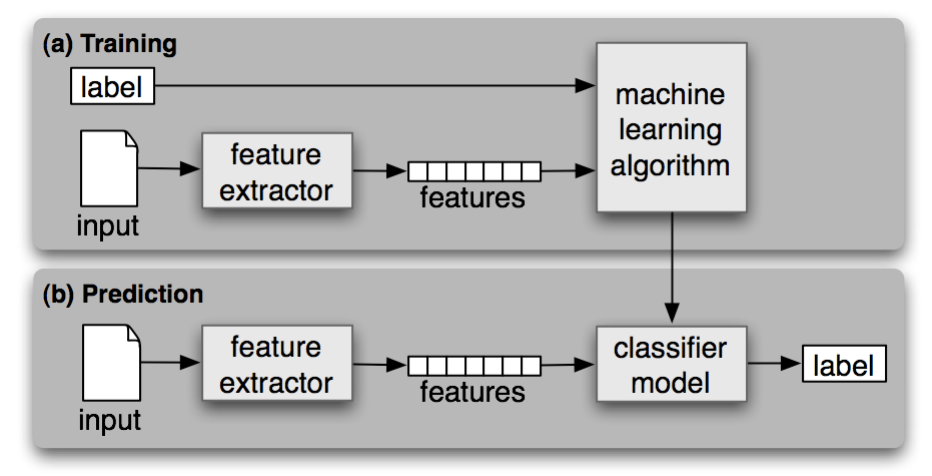
\includegraphics[width=0.8\textwidth]{process_flow.png}
\caption{Supervised Classification\protect\footnotemark}  
\cite{bird_natural_2009}
\end{figure}

\subsection{Maximum Likelihood Estimate and Bayes Theorem}
Express our idea using Bayesian probability terminology:
\begin{align*}
posterior  &\propto  prior \times likelihood
\end{align*}
When we compare the probability of different form for lemma $l_i$, we are comparing the $p(f_i|l_i)$, posteriors  of lemma $l_i$ predicted as form $f_i$. It depends on the prior of the form $f_i$ and the likelihood of the lemma $l_i$ when form $f_i$ shows.
\begin{equation}
\frac{p(f_i|l_i)}{p(f_j|l_i)} = \frac{p(f_i) \cdot p(l_i \mid f_i)}{  p(f_j) \cdot p(l_i \mid f_j) } \qquad \qquad  f_i,f_j \in Forms(l_i)
\end{equation}
And $p(f_i) \cdot p(l_i \mid f_i)$ can even be simplified if we apply the MLE estimator $\frac{f}{n}$ to it.
\begin{equation} 
\label{eq:simple_mle}
\begin{aligned}
\hat{p}(f_i) \cdot \hat{p}(l_i \mid f_i) &= \frac{freq(f_i)}{n} \cdot \frac{freq(l_i, f_i)}{freq(f_i)} \\
&= \frac{freq(l_i, f_i)}{n}
\end{aligned}
\end{equation}

The equation \ref{eq:simple_mle} is a simple theoretical model. It maybe a little astonishing that,based on this model, if we want to compare $p(f_i|l_i)$ and $p(f_j|l_i)$, just need to compare the co-occurrence $freq(l_i,f_i)$ and $freq(l_i,f_j)$.  The problem is we can't deal with those lemmas we haven't seen. Since we use NLTK package, the smooth method of NLTK will be given later on. 

The result of unigram MLE will be used as our baseline.

\subsection{Naive Bayes}
Naive Bayes is a classification technique based on Bayes' theorem with independence assumption.  given a problem instance to be classified, represented by a vector ${\mathbf  {x}}=(x_{1},\dots ,x_{n})$ representing some n features (independent variables), it assigns to this instance probabilities for each of K possible outcomes or classes $C_{k}$. \cite{murty_pattern_2011}

\[p(C_{k}\mid x_{1},\dots ,x_{n})={\frac {1}{Z}}p(C_{k})\prod _{i=1}^{n}p(x_{i}\mid C_{k})\]

With the the "naive" conditional independence assume that each feature $x_{i}$ is conditionally independent of every other feature $x_{j}$ for $j \neq i$, given the category. 

The prediction lemma-form problem, For Any given lemma $l_i$ we suppose that there is a form list $Forms(l_i)=\{f_{i1},f_{i2},...,f_{ik}\}$ which contains all its possible forms. The lemmas sequence $(l_1,l_2,...,l_n)$ are the sequence we can observe, so we take them as features. Then the form sequence is the classes that we want to put the features in\footnote{We will probably use both "label" or "class","tag" or "classify" in this notes, they will mean same thing.}. Actually,in this way,  we built up a label list contains all the forms show up in the corpus $\{Forms(l_1),Forms(l_2),..., Forms(l_n)\}$, the size of this list will be $V$, which is the total vocabulary of the forms in the corpus. Unfortunately, due to the immense of the vocabulary, the conditional probabilities table will be infeasible.

\[p(V|l_1,...,l_n) = \frac{1}{Z} p(V) \prod _{i=1}^{n}p(l_i \mid V) \]

Actually when we do predicting for the lemma $l_i$ in a sequence $(l_1,l_2,...,l_n)$, we just need to look at $Forms(l_i)$ and don't have to take account the $Forms(l_j)$ ($j \neq i$). In this section, We see the prediction of form for each lemma $l_i  \Longrightarrow f_i$ as a classification by choosing the labels only from $Forms(l_i)$. It's reasonable since the lemma is kind of the product of the lemmalization of the correspond forms $\{f_{i1},f_{i2},...,f_{ik}\}$. The one feature NB model correspond to our problem is like:

\[p(f_i|l_i) \propto p(f_i) \cdot  p(l_i|f_i)\]


And since one time training will prepare the parameters for the prediction for one lemma, if the train set contains $n$ different lemmas, then the model will be trained $n$ times. Nevertheless the same lemma will share the same parameters. So we use a dictionary to store them to avoid the the repetition work.


The bigram model we built is taking account the influence of the $l_{i-1}$ to $f_i$.
\begin{align}
p(f_i|l_{i-1},l_i) &\propto p(f_i) \cdot  p(l_{i-1},l_i|f_i)  \\
&= p(f_i) \cdot  p(l_{i-1}|f_i) \cdot p( l_i | l_{i-1},f_i) \label{eq:bigram_mod} \\
&= p(f_i) \cdot  p(l_{i-1}|f_i) \cdot p( l_i | f_i) \label{eq:bigram_nb}
\end{align}

Apply the Naive Bayes assumption to get from equation \ref{eq:bigram_mod} to \ref{eq:bigram_nb}. 

And in our case, if we see "of find" to the probability of classifying "find" into "finding"   it would be:
\begin{equation} \label{eq:bigram_find}
p(finding | of,find) \propto p(finding)\cdot p(of | finding) \cdot  p(find | finding)) 
\end{equation}
$form_i="finding" \quad lemma_{i-1}="of" \quad lemma_i="find"$ 


\subsection{Practical Work with NB}

Take the lemma "find" in file <dev-24> as an example(The first 90\% of the file is taken as the train set N=1576467). Table \ref{tb:cfd_find} shows the conditional frequency of the forms of "find" in the train set. 

\begin{table}[htb]
\centering
\begin{tabular}{|l|llllll|}
\hline
form $f_i$       & found & find & finds & finding & Finding & Finds \\ \hline
freq($f_i$,"find") & 778   & 204  & 65    & \textbf{32}      & 4       & 2     \\ \hline
freq($f_i$) & 778   & 204  & 65    & \textbf{45}      & 4       & 2     \\ \hline
\end{tabular}
\caption{conditional frequency of the forms of "find"}
\label{tb:cfd_find}
\end{table}

Although we don't even need to use the $freq(f_i)$ in our current model, it's for the future use.

Suppose our one feature NB model is classifying the lemma "find", the only feature is \{"lemma":"find"\} and the classes to be chosen from are \{found, find, finds, finding, Finding, Finds\}. The model will compare the max $p(f_i|l_i)$ and do the classification. No doubt, $p("found" | lemma="find")$ is the max, thus the classes will always be form "found". We call this unigram. Because this model just has one feature and only the $l_i$ will affect the classes $f_i$. 

\subsubsection{Smooth method of NLTK Naive Bayes}

According to the source code of NLTK class ELEProbDist which is the feature distribution function of NaiveBayesClassifier, it takes Expected Likelihood Estimate method, the probability distribution is given as below:\cite{loper_nltk.probability_nodate}
\begin{equation}
p(x_i)=\frac{C+0.5}{N+0.5B} \qquad X = \{x_1,x_2,\dots,x_o,\dots\}
\end{equation}

$C$ is the frequency we count with $N$ outcomes and $B$ the number of the observed value of $X$. 




\subsubsection{Training set}

We didn't notice this problem until we looked at the table \ref{tb:cfd_find}. The $freq("finding")=45$ is slightly bigger that the $freq("finding","find")=32$. That means the form "finding" correspond to other lemma other than "find", for example, lemma "finding". Then question is when we train the classifier for lemma "find", whether should we put the ("finding","finding") in the train data? Or we can put this question in another way, does ("finding","finding") show or not in train data affect the training result of the model?

We observe train data [("find","finds"),("find","finding"),("finding","finding")]\footnote{in the format (lemma, form)}. 
\begin{lstlisting}
m1 = [({'lemma':'find'},'finds'),({'lemma':'find'},'finding')]
m2 = [({'lemma':'find'},'finds'),({'lemma':'find'},'finding'),({'lemma':'finding'},'finding')]
b1 = [({'find':True},'finds'),({'find':True},'finding')]
b2 = [({'find':True},'finds'),({'find':True},'finding'),({'finding':True},'finding')]
\end{lstlisting}
\begin{align*}
p_{m1}^*('lemma':'find'|'finding')&=(1+0.5)/(1+1/2)=1 \\
p_{m2}('lemma':'find'|'finding')&=(1+0.5)/(2+2/2)=0.5 \\
p_{b1}('find':True|'finding')&=(1+0.5)/(1+1/2)=1 \\
p_{b2}('find':True|'finding')&=(1+0.5)/(2+2/2)=0.5
\end{align*}
*These values can be check by the \_feature\_probdist method of a classifier of class NaiveBayesClassifier. For example:
\begin{lstlisting}
classifier_m._feature_probdist[('finding', 'lemma')].prob('find')
classifier_b._feature_probdist[('finding', 'find')].prob(True)
\end{lstlisting}

For $p_{m1}$, $C$ equals to the count of feature 'lemma'='find' and classifier form 'finding' show up, which is 1 in this case. And $B$ is the number of the observed value of the feature name 'lemma', we just can see 'lemma'='find', so it's 1.
But after we add the ("finding","finding"), which corresponds to the feature. For $p_{m2}$, $C$ keeps unchanged. Though it has two possible values 'find' and 'finding' for feature 'lemma' now. So $B$=2.

Same situation for $p_{b1}$ and $p_{b2}$. But we should pay attention that in NLTK NaiveBayes model, it will complete the known features for every element with a None value if this feature doesn't show up in the current item. That means the td\_b2 will be completed as below:
\begin{lstlisting}
b2 =
[({'find':True,'finding':None},'finds'),
({'find':True,'finding':None},'finding'),
({'finding':True,'find':None},'finding')]
\end{lstlisting}

It shows us adding ("finding","finding") does matter the probability. Compare the train data set (2) to (1) for $l_i$. So those pairs which contain the forms of the current objective lemma added to the train set.
\begin{align*}
&train\_data\_set_{l_i} (1) = pairs_{l_{i}} = [ (l_{i},f_{i1})*freq(l_{i},f_{i1}),\dots,(l_{i},f_{ik})*freq(l_{i},f_{ik})] \\
&train\_data\_set_{l_i} (2)= \sum_{j} pairs_{f_{ij}} \\
&pairs_{f_{ij}}=[ (l_{j1},f_{ij})*freq(l_{j1},f_{ij}),\dots,(l_{jm},f_{ij})*freq(l_{jm},f_{ij}) ] \\ 
&f_{i1},\dots,f_{ik} \in Forms_{l_i} \\
&l_{j1},\dots,l_{jm} \in Lemmas_{f_{ij}} 
\end{align*}

Add the ("finding","finding") to the train data, to decrease the p(find|finding) it's like to tell the model that, if there are more form "finding" correspond to lemma "finding", then probably few correspond to lemma "find". 

\subsubsection{Feature format}
And take a look of this example below, it will show us the difference between the muti-value format feature and bi-value format feature. 

\begin{lstlisting}
m3 = [({'lemma':'find'},'finds'),({'lemma':'find'},'finding'), ({'lemma':'finding'},'finding'),({'lemma':'pseudo-f'},'finding')]
b3 = [({'find':True},'finds'),({'find':True},'finding'),
({'finding':True},'finding'),({'pseudo-f':True},'finding')]
\end{lstlisting}
\begin{align*}
p_{m3}=(1+0.5)/(3+3/2)=0.43 \\
p_{b3}=(1+0.5)/(3+2/2)=0.5 
\end{align*}


We set a pseudo lemma 'pseudo-f' for 'finding', we add the ('pseudo-f','finding'), the probability p(find|finding) dropped more quickly for the multi-value format feature. For the bi-value format feature, the $B$ value remains 2. But for the multi-value format feature, the $B$ value will grow as we add new lemmas, which will leave more possibility for the unseen situations. This difference won't be very huge for unigram, since most forms just have not more than 2 corresponded lemmas. Actually that's also why we have to set a pseudo lemma for "finding". But if we start to use bigram in the multi-value format feature, this difference is much bigger.

\subsection*{Bigram}

Before we implement the equation \ref{eq:bigram_find} for bigram, we face the problem then, how can we prepare the feature set to feed the NLTK Naive Bayes model? The feature is \{"lemma-1":"to","lemma":"find" \} or 
 \{"bigram":("to","find"),"lemma":"find" \}? Based on equation \ref{eq:bigram_find}. We have to chose \{"lemma-1":"to","lemma":"find" \}. But how about \{"to":True,"find":True \}?

Using equation \ref{eq:bigram_find}, We calculate the p(find|finding) for both multi-value and bi-value form feature for the train data in <dev-24> and listed in \ref{tb:cfd_find}:

The right part of equation \ref{eq:bigram_find} can be presented in 4 different forms in both multi-value and bi-value format feature. 

\begin{align*}
&(1)=p(finding) \cdot p("lemma-1":"of"|'finding') \cdot p("lemma"="find"|'finding') \\
&(2)=p(finding) \cdot p("of":True|'finding') \cdot p("find"=True|'finding') 
\end{align*}
\begin{align*}
p("lemma"="find"|'finding') &= (32+0.5)/(45+2/2) = 0.707 \\
p("find"=True|'finding') &= (32+0.5)/(45+2/2) = 0.707 \\
p("lemma-1":"of"|'finding') &= (2+0.5)/(45+316/2) = 0.012 \\
p("of":True|'finding') &= (2+0.5)/(45+2/2) = 0.054 
\end{align*}

The "of" shows 2 times in the bigrams of lemma for form finding. The types of the values in the name of "lemma-1" is 316. And it makes the p("lemma-1":"of"|'finding') value quite small. 
And of course, we don't know the difference of the classification result yet. Because when you compare the p('finding'|"lemma-1":"of","lemma":"find") and p('finds'|"lemma-1":"of","lemma":"find"), the latter will take exactly the same $B$ value, then it reduces the influence of the ratio.

The result proves result by using the multi-value format feature and bi-value format feature is very close.


\begin{table}[htp]
\centering
\begin{tabular}{|l|l|l|l|}
\hline
File           & Baseline  & Bigram multi-value & Bigram bi-value \\ \hline
dev-24         & 78.09\%    & 84.38\%            & 84.37\%         \\ \hline
dev-24...241   & 79.55\%    & 86.97\%            & 86.91\%         \\ \hline
\end{tabular}
\caption{Bigram accuracy of multi-value and bi-value format feature}
\label{bigram_nb}
\end{table}
\begin{itemize}
\item dev-24 (1 file) (1578267 itmes for training, and 175363 items for test)
\item dev-24...241 (10 files): dev-24,dev-25,dev-26,dev-27,dev-28,dev-237,dev-238,dev-239,dev-240,dev-241 (12176586 itmes for training, and 1352955 items for test)
\end{itemize}

And for the unigram, the model performs the same with two kinds of format feature on dev-24, it gives 78.07\%.


\subsubsection{Over-fitting?}
Actually for Naive Bayes, another advantage is that it's so simple, so few parameters to be trained. It makes it won't be trapped by the local maximum. So we believe that we don't need to worry about the over-fitting problem.


\section{Related work}
\subsection*{Lemma == Form}
The prediction of whether Lemma \& Form are identical. It's a simplified problem we tried to resolve. By using it test our models and ideas, we get a very short training and testing time and the performance of the result can also be a reference for the solution to the original problem. Because the performance of the original problem can never exceed the result of this simplified problem.

\begin{table}[htp]
\centering
\begin{tabular}{|l|l|l|l|}
\hline
       & unigram & bigram & trigram \\ \hline
dev-24 & 84.12\%   & 89.53\%  & 87,93\%   \\ \hline
\end{tabular}
\caption{Lemma == Form prediction}
\label{tb:lemma_eq_tb}
\end{table}

\subsection*{POS}
We believe that Part of Speech tagging will help to eliminate the ambiguity of the lemma, e.g. play as verb or as noun. Result shows it will slightly increase the accuracy but not more than 0.4\%, which is a little lower than we expected. The possible reason for this is: firstly, the lemmas who have the ambiguity between different kinds of POS tagging are not so many. Second, apply the real text trained POS tagging to lemma, it gives a relative lower performance also.

\subsection*{HMM}
Our first idea is to apply HMM to this problem. The output observation is the lemma sequence and the form sequence are hidden states. But after the trial of the HMM tagger in NLTK, and we found it's incredibly slow. A training model with only 2000 sentences predict incorrectly 5 words in about 5 minutes. 

\subsection*{Non-utf8}
The appearance  of the Non-utf8 will cause the code can't succeed to decode the corpus text in encoding "utf8". We found most of the non-utf8 characters show in lemmas and the non-utf8 characters byte minus the byte at correspond position in form equals 0x20. It's the value we usually use to get a uppercase letter to lowercase. So we guess the problem is caused by the program lemmalisation lowercased incorrectly some utf-8 letters. If the encoding "latin1" is used for both read and write the corpus file. The problem is ignored. Otherwise, if the encoding utf-8 is used to read the file. Since the non-utf8 will cause the error of the decoder, two situation will happen to the non-utf8 characters: ignore or replace. And both situation will cause the mismatching of the lemma and form. It will slight affect the accuracy of the prediction. 
Since we haven't done the complete statistics for these non-utf8 characters, the reason caused this problem remains a guess. But if the related work would like to be done by someone, We suggest the exception tackle mechanism in python to fix or count these non-utf8 characters. It seems very practical.  

\section{Discussion}
\subsection*{Smooth for unseen}
And if the bigram model encounter a unseen bigram pair, which means it will simply delete the new unseen feature.\cite{loper_nltk.classify.naivebayes_nodate} Thus for that pair, only the original lemma feature provide the information, in this situation, it's a unigram model.
If the model encounter a unseen lemma, we predict a identical form for it. That's out of the nltk Naive Bayes. 
\subsection*{Limit}
Due to the Naive Bayes Assumption, the features are independent. Then we ignore the influence between the lemmas. But it's not realistic. 

Additionally, since we classify the lemma one by one. In our model, we assume that for two lemmas $l_i$ and $l_{j}$, the prediction form $f_{i}$ is independent of every other $f_{j}$ for $j \neq i$. Obviously, it's not realistic. For example, the lemma series "student be", if the "student" is predicted as "students", then the "be" should be either "are" or "were".
\subsection*{Expected Likelihood Estimate}
The Naive Bayes Model is not trained in NLTK. But we have the reason to believe the ELE model or ELE technique is chosen specially for the classification task. 
The ELE model is the additive smoothing with the lambda = 0.5, comparing to Laplace estimation which is with the lambda = 1.
But we are still doubt that whether it's the best distribution for our case. More work should be done here.

\section{Conclusion}
Naive Bayes classifier in NLTK is capable of resolving the lemma-form prediction problem and gives us a good performance compare to the baseline. But its relatively fixed interface makes the user not easy to adjust the parameter to achieve a better performance.



\bibliographystyle{apacite}
\bibliography{jason,sample}
\end{document}